\documentclass[addpoints,12pt]{exam}
\newcommand{\ds}{\displaystyle}
\usepackage[margin=0.8in]{geometry}
\usepackage{subcaption}
\usepackage{tikz}
\usepackage{amssymb,amsmath,graphicx,wrapfig,verbatim,wasysym, enumitem,psfragx,color}
\usepackage{multicol}

\usepackage{pgf,tikz,pgfplots}
\usepackage{stmaryrd}
\usetikzlibrary{arrows, shapes.geometric, matrix, turtle, plotmarks}

%\usepackage{fancyhdr}
%\setlength{\headheight}{13.6pt}
%\pagestyle{fancy}
%\lhead{Math 222}
%\chead{ Midterm 1 }
%\rhead{Spring 2022}

\def\FillInBlank{\rule{3truein} {.01truein}}




% Choose one option (bubbles)
\newcommand{\chooseone}{{\Large$\Circle$\ \ }}
% Choose multiple options (squares)
\newcommand{\choosemany}{{\Large$\Square$\ \ }}


\newcommand{\myleft}{\makebox[.4\textwidth]{First Name:\enspace\hrulefill}}
\newcommand{\myright}{\makebox[.4\textwidth]{Last Name:\enspace\hrulefill}}
\header{\oddeven{\myleft}{}}
    {}
    {\oddeven{\myright}{}}

\footrule

\footer{Math 211}
     {Midterm 1 - Fall 2024}

    {Page \thepage\ of \numpages}

\begin{document}

\begin{questions}

\question Clearly mark the correct answer(s) for each of the following by completely filling in the
appropriate bubble. \textbf{No justification is needed.}




\begin{parts}




\part[2] \textbf{(Multiple Choice-Choose one)} Let $f(x)$ and $g(x)$ be two functions such that
$f(2) = -3$, $g(2) = 7$, $f'(2) = 3$, $g'(2) = 10$, and $f'(7) = 4$. Which of the following is the
instantaneous rate of change of $f(g(x))$ when $x = 2$?

\begin{itemize}[label={}]
\item \chooseone 3
\item \chooseone 30
\item \chooseone 40
\item \chooseone 210
\item \chooseone None of the above.
\end{itemize}


\vfill


\part[2] \textbf{(Multiple Choice-Choose one)} Suppose $f(t)$ represents the temperature $t$
hours after noon. Suppose the temperature at 3:00pm ($t = 3$) is rising increasingly rapidly.
Which of the following is true?
      \vspace{0.15in}
\begin{itemize}[label={}]
\item \chooseone $f'(3)$ is negative, while $f''(3)$ is positive.
\item \chooseone $f'(3)$ is positive, while $f''(3)$ is negative.
\item \chooseone $f'(3)$ and $f''(3)$ are both positive.
\item \chooseone $f'(3)$ and $f''(3)$ are both negative.
\end{itemize}

\vfill




\part[2] \textbf{(True/False)} Suppose $g(x)$ is a function with $\displaystyle\lim_{ x \to 4^+}
g(x) = 1$, $\displaystyle\lim_{x\to 4^-}g(x)=2$, and $g(4) = 2$. Then $g(x)$ is continuous at
$x=4$.

\begin{itemize}[label={}]
\item \chooseone True
\item \chooseone False
\end{itemize}

\vfill


\newpage




\part[2] \textbf{(Multiple Choice-Choose one)} Which of the following is equal to
$\dfrac{10}{\sqrt[3]{8x^2}}$?
\begin{itemize}[label={}]
\item \chooseone $20x^{6}$
\item \chooseone $20x^{-3/2}$
\item \chooseone $5x^{-3/2}$
\item \chooseone None of the above.
\end{itemize}

\vfill


\part[2] \textbf{(Multiple Choice-Choose one)} What is the domain of the function\\ $y=f(x)$
shown below?

\begin{minipage}{.4\textwidth}
\begin{itemize}[label={}]
\item \chooseone $[1,6]$
\item \chooseone $[-2,5]$
\item \chooseone $(-2,2)\cup(2,5)$
\item \chooseone $[-2,2)\cup(2,5]$

\item \chooseone None of the above.
\end{itemize}
\end{minipage}
\begin{minipage}{.5\textwidth}
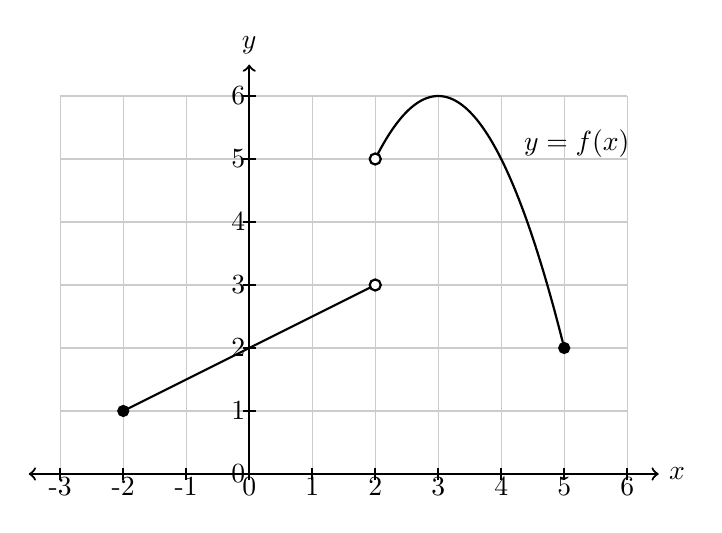
\begin{tikzpicture}[scale=.8]
\draw[gray!40] (-3, 0) grid[step=1] (6, 6);
\draw[<->,thick,black] (-3.5,0)--(6.5,0) node[right]{$x$};
\draw[->, thick,black] (0,0)--(0,6.5) node[above]{$y$};
\foreach \x in {-3,-2,...,6}
\draw[thick] (\x,-.1) --(\x,.1) node[below]{\x};
\foreach \y in {0,1,...,6}
\draw[thick] (-.1,\y) --(.1,\y) node[left] {\y};
\draw[domain=2:5,samples=100, thick,-] plot ({\x},{-(\x-3)^2+6});
\draw[domain=-2:2,samples=100,thick,-] plot ({\x},{\x/2+2});
\draw[fill=black] (5,2) circle[radius=0.25em];
\draw[fill=white,thick] (2,3) circle[radius=0.25em];
\draw[fill=white,thick] (2,5) circle[radius=0.25em];
\draw[fill=black] (-2,1) circle[radius=0.25em];
\node at (5.2,5.25) {$y=f(x)$};
\end{tikzpicture}

\end{minipage}
\vfill

\end{parts}

\newpage


\question Calculate the derivative of each function. You do not need to simplify your answers.

\begin{parts}

\part[5] $f(x)=(x^3+2x-1)(x^2-10x)$

\vfill




\part[5] $g(x)=\dfrac{2}{7x^2}+3x^4+\sqrt{2}$

\vfill

\part[5] $r(t)=\sqrt[4]{t^2+t}$




\vfill


\part[5] $F(x)=(2x^6+x^2)^9+3x$




\vfill

\end{parts}

\newpage




\question For the graph of $y=f(x)$ below:

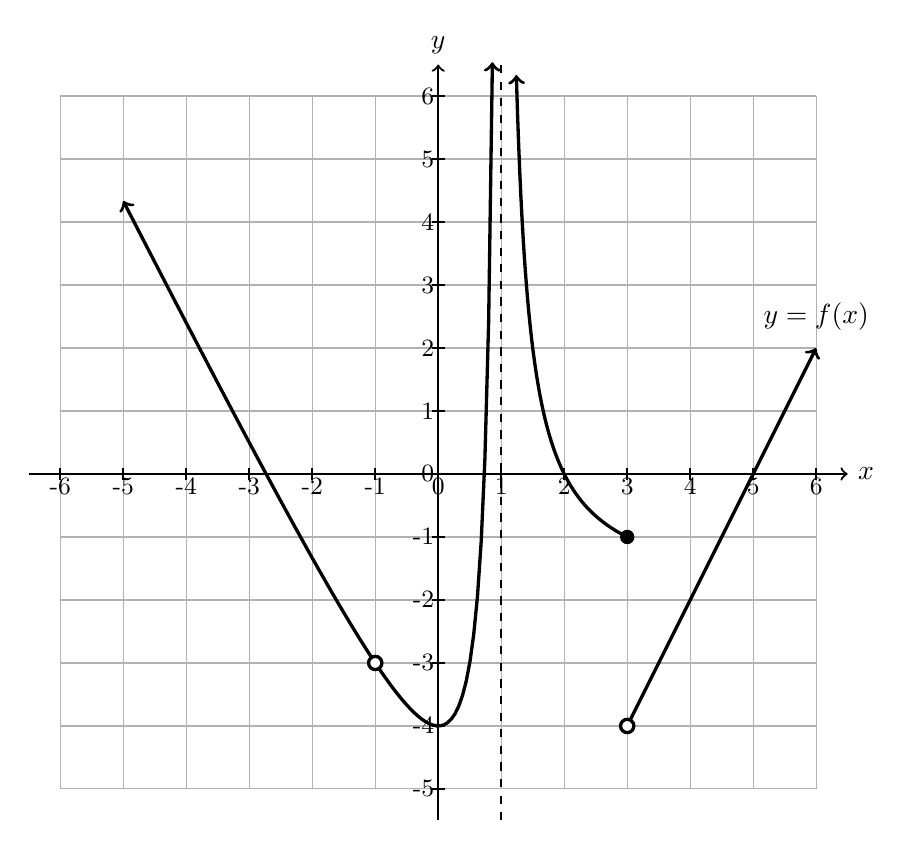
\begin{tikzpicture}[scale=0.8]
\draw[gray!60] (-6, -5) grid[step=1] (6, 6);
\draw[->,thick,black] (-6.5,0)--(6.5,0) node[right]{$x$};
\draw[->, thick,black] (0,-5.5)--(0,6.5) node[above]{$y$};
\foreach \x in {-6,...,6}
\draw[thick] (\x,-.1) --(\x,.1) node[below] {\small \x};
\foreach \y in {-5,...,6}
\draw[thick] (-.1,\y) --(.1,\y) node[left] { \small \y};
\draw[domain=-5:0.86,samples=100, very thick,<->] plot ({\x},{-2*\x*\x/(\x-1)-4});

\draw[domain=1.24:3,samples=100, very thick,<-] plot ({\x},{2/(\x-1)-2 });
\draw[domain=3:6, samples=100, very thick, ->] plot ({\x}, {2*\x-10});
\draw[fill=black] (3,-1) circle[radius=0.3em];
\draw[fill=white,very thick] (-1,-3) circle[radius=0.3em];
\draw[fill=white,very thick] (3,-4) circle[radius=0.3em];
\node at (6,2.5) {$y=f(x)$};
%\draw[thick,dashed] (-2,-4)--(-2,4);
\draw[thick,dashed] (1,-5.5)--(1,6.5);
\end{tikzpicture}

\begin{parts}

\part[3] For which $x$-value(s) is $f(x)$ discontinuous?

\vspace{0.75in}


\part[6] Find each limit, if possible (use $+\infty$ or $-\infty$ if applicable). If not possible, write
DNE.
\vfill

(a) $\displaystyle \lim_{x\to -1} f(x)=$

\vfill

(b) $\displaystyle \lim_{x\to 1^-} f(x)=$
\vfill

(c) $\displaystyle \lim_{x\to 3^{-}} f(x)=$

\vfill

(d) $\displaystyle \lim_{x\to 3^{+}} f(x)=$
\vfill

(e) $\displaystyle \lim_{x\to 3} f(x)=$
\vfill

(f) $\displaystyle \lim_{x\to 4} f(x)=$




\end{parts}

\newpage

\question[8] Find $f''(x)$ for $f(x)=12\sqrt{x}(x+1)$. You do not need to simplify your final
answer. Show all work.

\newpage

\question Suppose a table manufacturer determines that their cost function $C(x)$ (in dollars)
for producing $x$ tables is $C(x)=30x+50$, while their revenue function $R(x)$ (in dollars) for
selling $x$ tables is $R(x)=45x-x^2$.

\begin{parts}

\part[5] Find the \textbf{profit function} $P(x)$, then find the $x$-value(s) where $P(x)=0$. Show
all work.

\vspace{2in}

\part[5] Find the \textbf{marginal revenue function} and evaluate it at $x=10$. You do not need
to simplify your numerical answer. Show all work.

\vspace{2in}

\part[2] Find the \textbf{average cost function}.

\vspace{1in}

\part[5] Find the \textbf{marginal average cost function} and evaluate it at $x=10$. You do not
need to simplify your numerical answer. Show all work.
\end{parts}

\vspace{2in}

\newpage

\question[11] Use the limit definition of the derivative to compute $f'(x)$, where $f(x)=2x^2-6x$.
Show all work.


\newpage

\question

Find each limit. Show all work. Simplify your final answers.

\begin{parts}
  \part[5] $\displaystyle \lim_{x\to 3} \dfrac{x^2+x-12}{2x-6}$

  \vfill

  \part[4] $\displaystyle \lim_{x\to 0}\dfrac{x^2+5x+4}{x^2+3x-4}$

  \vfill
\end{parts}

\newpage


\question[10] Find an equation for the tangent line of $f(x)=x^4+2x+4$ at $x=-1$. Show all work.


\newpage




\question Consider the function $y=f(x)$ below. Clearly mark the correct answer(s) for each of
the following by completely filling in the appropriate bubble. \textbf{No justification is needed.}
​
​         \begin{tikzpicture}[scale=.99]
​         ​       \draw[gray!60] (-5, -5) grid[step=1] (5, 5);
​         ​       \draw[<->,thick,black] (-5.3,0)--(5.3,0) node[right]{$x$};
​         ​       \draw[<->, thick,black] (0,-5.3)--(0,5.3) node[above]{$y$};
​         ​       \foreach \x in {-5,-4,...,5}
​         ​       \draw[thick] (\x,-.1) --(\x,.1) node[below] {\small \x};
​         ​       \foreach \y in {-5,-4,...,5}
​         ​       \draw[thick] (-.1,\y) --(.1,\y) node[left] {\small \y};
​         ​       \draw[domain=-4.75:4.25,samples=200,very thick,<->] plot
({\x},{(\x-2)^2*(\x+4)/8});
​         ​       \node[thick] at (5,3.25) {$y=f(x)$};
​         \end{tikzpicture}


\begin{parts}
\part[2] \textbf{(Choose all that apply)} For which $x$-value(s) is $f'(x)=0$?
\begin{itemize}[label={}]
\item \choosemany $x=-4$
\item \choosemany $x=-2$
\item \choosemany $x=2$
\item \choosemany $x=4$
\end{itemize}

\vfill

\part[2]\textbf{(Multiple Choice-Choose one)} Is $f'(-3)$ positive, negative, or zero?
\begin{itemize}[label={}]
\item \chooseone positive
\item \chooseone negative
\item \chooseone zero
\end{itemize}
\vfill


\part[2]\textbf{(Multiple Choice-Choose one)} Is $f'(1)$ positive, negative, or zero?

\begin{itemize}[label={}]
\item \chooseone positive
\item \chooseone negative
\item \chooseone zero
\end{itemize}

\end{parts}
\vfill

\end{questions}

\end{document}
